\documentclass[11pt,letterpaper]{article}
\usepackage[T1]{fontenc}
\usepackage{lmodern,microtype,amsmath,amssymb,amsthm,booktabs,tabularx,array,graphicx,xcolor,fancyhdr}
\usepackage[margin=0.94in,headheight=15pt]{geometry}
\definecolor{ink}{HTML}{183548}
\definecolor{teal}{HTML}{166D6B}
\usepackage[colorlinks,linkcolor=teal,urlcolor=teal,citecolor=teal,pdftitle={Post-Acceptance Research Investigations in Learning-Augmented Cache Eviction},pdfauthor={Soroush Vahidi},pdfsubject={Technical report on exact counterfactual evaluation, supervision, and selective eviction}]{hyperref}
\graphicspath{{../figures/}}
\pagestyle{fancy}
\fancyhf{}
\fancyhead[L]{\small\textcolor{ink}{Post-acceptance research in cache eviction}}
\fancyhead[R]{\small\textcolor{ink}{November 2026}}
\fancyfoot[C]{\thepage}
\newtheorem{theorem}{Theorem}
\newcolumntype{Y}{>{\raggedright\arraybackslash}X}
\newcommand{\code}[1]{\texttt{\detokenize{#1}}}
\newcommand{\boundarynotice}{This report documents research investigations conducted after the acceptance of the original Knowledge-Based Systems manuscript on November 15, 2026. These investigations are separate from the experiments reported in the accepted manuscript and have not undergone the manuscript\textquoteright s peer-review process.}

\begin{document}
\hypersetup{pageanchor=false}
\begin{titlepage}
\thispagestyle{empty}
\raggedright
\vspace*{0.72in}
{\large\textcolor{teal}{Technical report \quad / \quad November 25, 2026}\par}
\vspace{0.35in}
{\color{ink}\Huge\bfseries Post-Acceptance Research Investigations in Learning-Augmented Cache Eviction\par}
\vspace{0.25in}
{\color{teal}\LARGE Exact Counterfactual Evaluation, Supervision, and Selective Eviction\par}
\vspace{0.53in}
{\Large Soroush Vahidi\par}
{New Jersey Institute of Technology\par}
\vfill
\rule{\textwidth}{0.45pt}
\vspace{0.14in}

\boundarynotice

\vspace{0.12in}
\textit{Original article.} Decision-aligned eviction-value prediction for learning-augmented caching. \textit{Knowledge-Based Systems}, 356, 117353. \href{https://doi.org/10.1016/j.knosys.2026.117353}{DOI 10.1016/j.knosys.2026.117353}.
\end{titlepage}
\hypersetup{pageanchor=true}

\begin{abstract}
Finite-horizon eviction supervision can leave most cache residents tied while still producing expensive and harmful online policies. This report consolidates completed experiments on causal eviction features, stateless and recurrent learners, and selective departures from least recently used (LRU) replacement. For unit-size fully associative paging, a virtual capacity-\(C+1\) LRU stack evaluates every forced victim under deterministic LRU continuation in expected \(O(C+H)\) time for a suffix of \(H\) requests and \(O(C)\) auxiliary space. A single alternative costs at most one additional miss relative to the LRU victim and at least \(\max(1,C-H)\) actions are optimal. The strongest controlled histogram-boosting finalist saved 3,730 of 565,126 LRU misses (0.660\%) on 840,000 retrospective scored requests at 18.35 times LRU CPU cost. No finalist satisfied the complete advancement screen. Independent confirmation stayed sealed.
\end{abstract}

\section*{Executive summary}
\addcontentsline{toc}{section}{Executive summary}
\begin{itemize}
\item The exact labeler turns exhaustive counterfactual LRU replay into a shared scan. Recorded correctness checks had zero unexplained mismatches and steady-state median speedups of 19.7\(\times\) over compiled exhaustive replay and 24.4\(\times\) over Phase 2A paired replay. Compiled exhaustive replay wins in some small cells.
\item Three narrow, distinct questions run through the evidence: whether a forced action has measurable upside, whether causal features predict that upside, and whether acting on those predictions improves the policy's evolving cache. Label discrimination and fixed-state shortlist coverage improved more consistently than closed-loop miss counts.
\item Fully resolved labels exposed additional profitable candidates. Larger datasets and longer horizons gave nonmonotonic or mixed policy results. Compact history and explicit benefit/risk estimates gave positive matched contrasts. Recurrent finalists underperformed LRU on the full retrospective grid.
\item Approximate ties and validation-calibrated abstention improved some boosting and DeepSets replays. All fifteen matched random runs beat the Ridge finalist, while calibrated boosting beat its own fifteen. The best boosting finalist incurred 31.50 CPU microseconds per request. The preliminary abstention configuration used 11.78 times LRU CPU and saved 3,702 misses.
\end{itemize}
\clearpage
\begingroup
\small
\tableofcontents
\endgroup
\clearpage

\section{Introduction and relationship to the accepted manuscript}
{\setlength{\emergencystretch}{2em}\boundarynotice\par}

The original paper by Vahidi~\cite{vahidi} studies finite-horizon eviction-value prediction and evaluates the deployed \code{evict_value_v1} pipeline under corrected leave-one-family-out comparisons. Its negative learned-policy result, Common-Model V2, tie-aware oracle, continuation and distribution-shift controls, and timing are preserved in the reviewer verification and archived tables. The accepted package's audited source is the October R3 revision.\footnote{\code{b7c2dd4707a387fd2e76b84b7a05a67df00c61e3}.} The packaged TeX and PDF were checked by digest. The October R3 package carries the final manuscript files, while the R2 reviewer materials retain the compact science and verification detail. Crossref assigns the article to volume 356, January 2027. The DOI registration and repository publication announcement are from November 2026.

The studies below reuse the historical workload suite and, in some controls, earlier published counts or frozen models. New execution records, mathematical statements, and scientific outcomes are identified by campaign. Published reference numbers retain their published interpretation.

\section{Chronological research overview}
\begin{tabularx}{\linewidth}{@{}>{\raggedright\arraybackslash}p{0.15\linewidth}>{\raggedright\arraybackslash}p{0.20\linewidth}Y@{}}
\toprule
Date (2026) & Evidence & Scope \\ \midrule
Aug.--Oct. & KBS R2/R3 and September PE work & Manuscript evidence plus separate historical exploratory work. Recovered counts, checkpoints and tie-census records retain historical provenance. \\
Nov. 21 & Neural terminal marker & Matched H4 pilot and full H4/8/16 MLP, DeepSets, pointwise and native replay. The committed five-fold startup snapshot is superseded by the terminal tables. \\
Nov. 24 & Phase 1 terminal receipt & Expanded causal features, global and object recurrence, static controls, ordered history and state interventions. \\
Nov. 24--25 & Phase 2A reducer and census & Existing-data audits plus new matched-state forced-action, paired-rollout, shortlist, censoring and compression measurements. \\
Nov. 25 & Phase 2B manifests & Shared LRU proof, correctness and benchmarks, matched students and renewed frozen-checkpoint fallback comparisons. \\
Nov. 25 & Phase 2C-A Slurm receipts & Grouped exact supervision, diagnostics, storage and cross-platform parity. \\
Nov. 25 & Phase 2C-B Slurm receipts & Production scaling, horizons/features, components/shortlists, gates/controls and inference profiling. \\
\bottomrule
\end{tabularx}

\section{Research questions and hypotheses}
\begin{enumerate}
\item Can permutation-equivariant scoring exploit the eviction decision set? The neural comparisons test ranking objectives, set scoring, fixed horizons and fallback on matched decisions and closed-loop replays.
\item Does explicit temporal state improve decisions? Expanded-feature controls and recurrent variants test recent events, global sequence context, object memory and state carry. Frozen retrospective replays assess the resulting policies.
\item Are ties, repeated feature groups, and ambiguous labels a practical supervision constraint? Stratified exact and approximate signatures, rank diagnostics, horizon sweeps and paired action costs test different aspects of that question.
\item Can inexpensive exact counterfactuals improve learning? Phases 2B and 2C compare fixed and fully resolved labels with common candidates, model families, sample sizes and controls.
\item Does selective eviction offer a defensible improvement over LRU? The advancement screen requires gains across families, comparison with matched controls and feasible measured CPU cost.
\end{enumerate}

\section{Datasets and evaluation protocols}
The historical development families are BrightKite, Citi Bike, Alibaba Block, MetaCDN, MetaKV, Twemcache and Wiki2018. The protocol uses the internal key \code{cloudphysics} for Alibaba Block. Use 32, 64 and 128 unit-sized slots, an empty start, 10,000 warm-up requests and 40,000 scored requests per cell. The 21 cells contribute 840,000 scored requests. The same trace can appear at multiple capacities, so cells are dependent. The protocol records exact trace identities, five training families and one designated validation family per outer fold. Phase 2C-B freezes validation selections before opening the outer replay stream. Normalization and feature masks are fit on training rows. All candidate rows of a state remain grouped. Independent confirmation inputs and outcomes remain sealed.

A fixed-state score considers one forced first victim, then a specified continuation, from a shared state. A closed-loop score advances the compared policy's own state at every request. Policy-generated ghost metadata, recent accesses and visit state therefore change along different replay trajectories. Hindsight variants have future information and supply headroom estimates. They are ineligible as causal deployment comparators.

Define \(M_p\) and \(M_0\) as the scored misses of policy and LRU. Positive relative reduction denotes fewer misses, \((M_0-M_p)/M_0\). The macro result averages family-relative reductions with equal weights. Leave-one-family-out sensitivity recomputes the pooled reduction with a family removed. CPU ratios specify the timing harness and its own LRU denominator. Aggregate counts have no confidence interpretation from treating the 21 cells as independent.

The five-family LAFC-Evict v1.0 candidate dataset uses a distinct pipeline, temporal splits and additional capacity 256~\cite{lafc}. It shares trace lineages with the retrospective grid. The forensic enumeration is a new analysis of existing release data. The release's absent BrightKite and Citi Bike families remain outside its licensing scope.

\section{Neural eviction and recurrent models}
\subsection{November stateless neural comparison}
The pointwise MLP maps one resident vector to a score. The DeepSets-style model~\cite{deepsets} conditions resident scores on pooled candidate context. Training contrasts included expected action regret and a regression-only set control. The seed-7 H4 pilot used 2,560 training groups and 256 validation groups. On the BrightKite 32-slot holdout, DeepSets saved 73 misses (14,353 vs. 14,426), and MLP increased misses to 23,185. DeepSets and the oldest victim each attained zero offline regret across all 403 sampled decisions. The pilot had 165 all-tie states and no unique optimum. DeepSets cost 86.97 CPU microseconds/request versus 0.67 for LRU on this pilot.

The full replay records 21-cell totals at H4, H8 and H16, with 133 neural fits and 42 traditional refits in the forensic inventory. It compares exact argmin and the 0.05 LRU near-tie margin for seed 7, plus seeded controls. DeepSets H8 seed 7 took 565,462 misses at argmin and 565,245 with the margin, versus 565,126 for LRU. Seed 19 at H8 argmin took 569,422. H16 seed 7 margin took 567,206 and H4 seed 7 margin took 567,079. H4 seed-7 MLP margin took 588,344. For H8 seed 7, the margin saved 217 misses compared with exact argmin. A matched seed-19 margin replay is absent from November. On 1,176 common LRU states, the near-tie policy disagreed in 1,009 groups, with 1,007 neutral, one beneficial and one harmful under resolved LRU continuation. These fixed-state counts do not attribute the policy's closed-loop changes. Matched native controls were newly replayed. LRB, 3L-Cache, CACHEUS, HALP and historical original-model results are retrieved controls when the archived table marks them as historical.

\subsection{Global state, object state and matched probes}
The expanded representation combines resident/item history, request-stream context and bounded ghost state. Phase 1 compared static expanded DeepSets and flat history models, global recurrence, object recurrence, dual GRU, and dual LSTM. Fixed small-window controls, recomputed state, reset and delayed or permuted sequences probe whether chronology and hidden-state carry explain any gain. The six-cell development reset yielded 18,097 misses versus 18,432 for its stateful parent. The permuted history control yielded 17,923 versus 18,464 for delayed chronological history. Targeted aggregation yielded 18,133 versus 18,205 for uniform. LRU yielded 16,949 on those development cells. Differences do not isolate the contribution of state carry or targeted aggregation independent of optimization exposure.

The terminal receipt verified 77 fits, 154 selected/latest hashes, and 548 replay records, including 63 native control replays matching the archive. Fixed dual GRU T03 gave 672,786 misses (19.05\% above LRU). Frozen finalist seeds 7, 19 and 42 gave 694,148, 706,244 and 708,103. Expanded DeepSets and dual LSTM gave 709,567 and 710,014. Seed-7 finalist offline discriminative accuracy was 60.59\% versus 57.58\% for fixed T03, with 21,362 more closed-loop misses. Median fixed T03 CPU was 613.87 microseconds per request, including 44.89 for recurrent updates. The corresponding native LRU median was 1.11. Median p95 eviction latency was 782.44 microseconds. The archived fixed T03 is a retrospective portfolio, while the frozen finalist applied the fold-specific selection rule.

\section{Feature redundancy, information and aliasing}
Phase 2A's complete November census covered 704,122 decisions and 51,806,208 candidate rows. Within-cell exact input repeats beyond the first occurrence accounted for 29.90\% of groups. Exact input-target repeats were 29.71\%, 29.56\% and 29.30\% at H4, H8 and H16. At H16, 29.51\% were in buckets with more than one target vector. Within-group candidate distinction can coexist with repeated whole groups. The repeated-group fraction ranged from near zero for several families to 99.98\% on Wiki2018.

On 6,720 matched decisions, legacy numerical rank ranged from 2--4 within cells at relative tolerance \(10^{-6}\), versus 6--48 for expanded candidates. Pooled ranks were 5/26, 48/50 and 13/14 for legacy, expanded candidates and request features respectively. Log transforms and scaling affect measured spectra. At H16, repeated same-input bucket membership fell from 1,228 to 1,029 to 1,011 with expanded features and added request context. Within those remaining repeated buckets the conditional value variance fell from 0.02821 to 0.00630 to 0.00196. The subsets differ by representation. At the matched sample's H16, the repeated-bucket disjoint-optimum rate and mean in-sample minimum regret were zero. Three earlier-to-later lookup policies and LRU fallback each had 0.00980 later per-decision regret. A bounded approximate neighbor search at normalized radius 0.15 found neighbors for 834/2,347 later legacy decisions versus 375 and 373 under the richer representations.

The separate LAFC v1.0 enumeration verified 277,995,072 candidate rows over 168 partitions and 2,363,286 physical decision groups across horizons. Within-partition exact input repetition was 32.81\%, input-target repetition 32.47\%, and membership in conflicting input buckets 27.60\%. The physical split keys were disjoint. That check neither establishes independent lineages nor tests every possible supervision window at a split boundary. Retaining multiplicities preserves the original empirical objective under exact group compression. Changing weights or sampling changes the estimand.

\section{Counterfactual supervision and horizon degeneracy}
A fixed prefix suppresses distinctions whose causal effect appears after its boundary. The full November reconstruction gave 487,226, 434,486 and 397,221 all-tie decisions at H4, H8 and H16 out of 704,122. The mean optimal-set fractions were 99.20\%, 98.69\% and 97.95\%, so uniform optimal-set accuracy can be high with little decision information. In a separate time-stratified Phase 2A sample, H4 through H32 tie rates declined from 58.93\% to 41.67\%. At H32, 96.23\% of candidates were optimal on average and LRU was optimal in 97.96\% of states.

Forced-action optimal paging uses a best possible future policy from each initial cache (Belady/MIN)~\cite{belady,mattson}. Its action regret relative to the best forced action answers a different question from the baseline-relative advantage when all branches continue with LRU. Shortlist screening uses the fraction of profitable states it covers and the fraction of attainable gains it captures. Censoring matters for reuse supervision: 6.05\% of Phase 2A candidates had unknown reuse status within 32 capacity units because the observed trace ended. Finite-trace non-reuse does not establish a true infinite reuse distance.

\section{Exact shared LRU labeler}\label{sec:algorithm}
At a full miss, let the \(C\ge1\) distinct residents be \((a_0,\ldots,a_{C-1})\), oldest first. Mandatorily admit a distinct incoming object \(z\). Evict one resident, then execute deterministic LRU. All costs count misses strictly after admission. Let \(M_x(h)\) be the absolute suffix misses when resident \(x\) was evicted and let
\[
 A_x(h)=M_{a_0}(h)-M_x(h)
\]
be its signed advantage against the reference first victim \(a_0\). The virtual stack is initialized as \((a_0,\ldots,a_{C-1},z)\). Its capacity is \(C+1\). The front boundary is \(b\), and the \(C\) remaining entries constitute the reference \(R\). Store \(b\), an ordered hash map for \(R\), a map of active initial victims to their output slots, and an initially zero integer \(B\) counting reference misses that hit \(b\).

\begin{table}[ht]
\centering
\begin{tabularx}{\linewidth}{@{}p{0.22\linewidth}XX@{}}
\toprule
Event & Shared update & Resolution \\ \midrule
Request \(y\in R\) & Move \(y\) to MRU. \(B\) and the reference miss count stay fixed. & If \(y\) is active, record \(A_y=B-1\). \\
Request \(y=b\) & Increment reference misses and \(B\). Make old reference LRU the new boundary. Append \(y\) at MRU. & If new boundary \(x\) is active, record \(A_x=B\). \\
Request \(y\notin R\cup\{b\}\) & Increment reference misses. Make old reference LRU the new boundary. Append \(y\) at MRU. & If new boundary \(x\) is active, record \(A_x=B\). \\
\bottomrule
\end{tabularx}
\caption{Shared continuation transitions. Resolved alternatives stay resolved. At each snapshot, assign \(B\) to active alternatives and zero to the reference.}
\label{tab:algorithm}
\end{table}

At any requested horizon emit the frozen values and shared active value, then reconstruct absolute \(M_x=M_{a_0}-A_x\). The implementation supports horizon zero, explicit horizon snapshots, observed-trace truncation and early resolution. Full absolute suffix labels require scanning reference misses through the requested endpoint. Relative labels may stop once every branch resolves if no later absolute snapshot is required.

\section{Mathematical results and scope}
\begin{theorem}[Deletion invariant and exactness]
Before resolution of an alternative \(x\ne a_0\), its ordered cache equals the virtual LRU stack with \(x\) deleted and \(A_x=B\). It becomes the reference after its event in Table~\ref{tab:algorithm}.
\end{theorem}
\begin{proof}
After admission the alternative contains \(b=a_0\) and omits \(x\). The invariant and \(B=0\) hold. On a hit in \(R\) to any object other than \(x\), moving that object to MRU commutes with deletion. On a hit to \(x\), the alternative misses, evicts its oldest \(b\), inserts \(x\), and reaches the reference order at advantage \(B-1\). On a request to \(b\), the alternative hits and the reference misses, so \(B\) increments. In the new virtual list the previous reference LRU is the boundary. On an outside request, both miss and the alternative evicts the old boundary. The new boundary is again the previous reference LRU, with \(B\) unchanged. In either miss event the deletion representation persists. If the new boundary equals \(x\), deleting it already gives the reference, resolving that alternative at \(B\). This covers every transition.
\end{proof}

\begin{theorem}[Cost bound, tight optimal multiplicity and coalescence]
For a prefix of length \(H\), every alternative adds at most one miss relative to the reference. At least \(\max(1,C-H)\) victims minimize suffix misses, and the bound is tight. After \(C\) distinct future requests, all ordered branches coincide and accumulated advantage stays constant.
\end{theorem}
\begin{proof}
Each alternative has advantage \(B\) while active and resolves at \(B\) or \(B-1\) for a nonnegative, nondecreasing \(B\). Thus \(A_x\ge-1\). With residents \((a,b)\), incoming \(z\) and suffix \((b)\), evicting \(b\) adds one miss.

For \(H<C-1\) at least one alternative remains active because each request resolves at most one. The final \(B\) is maximal. If \(B=0\), the reference attains it and at most \(H\) resolved alternatives fall below. If \(B>0\), the last boundary-hit step can resolve at most one alternative and that alternative attains the final \(B\). At most \(H-1\) alternatives fall below, and the reference adds one more. For \(H\ge C-1\) existence of a minimizer gives the bound. For \(H\le C-1\), request \(H\) distinct nonbaseline residents once each: precisely those \(H\) first-eviction choices incur one extra miss. For longer \(H\), use the \(C-1\)-request construction and repeat its final request. When \(C=1\), the sole action is optimal.

After observing \(C\) distinct future objects, each ordered cache is the last \(C\) distinct requests in recency order, independent of its initial state. Equal ordered caches at the same cursor experience identical deterministic updates and miss increments. Repeating the incoming object shows that request count alone cannot guarantee coalescence for \(C\ge2\).
\end{proof}

Initialization and one full vector cost \(O(C)\). Each request uses expected \(O(1)\) operations under hash-table assumptions. Core work is expected \(O(C+H)\) and live state is \(O(C)\). \(q\) explicit snapshots cost an additional \(O(qC)\) output work and retained output memory, plus horizon bookkeeping. Ordered-map object overhead is implementation dependent. The optional distinct-object diagnostics also retain seen IDs over the observation range. With distinct-object stopping, some individual alternatives can resolve earlier. Ending a trace before coalescence gives an exact observed-prefix label and leaves unobserved effects unidentified.

\paragraph{Benefit and risk.} With fixed deterministic LRU continuation, \(A_x\) is integral and bounded below by \(-1\). Thus
\[
 A_x=\max(A_x,0)-\mathbf 1\{A_x=-1\},
 \qquad
 \mathbb{E}[A_x\mid X]=\mathbb{E}[\max(A_x,0)\mid X]-\Pr(A_x=-1\mid X).
\]
This net decomposition is one representation. The algorithm also records gross prevented reference misses (boundary hits before resolution) and the indicator of a branch-only miss (a request to the active omitted object). Their difference is exactly \(A_x\), and both gross components can be positive for one alternative. Phase 2C-B fits those gross components, subtracts estimated risk from estimated benefit, and evaluates a risk cap. Prediction error, candidate distributions, and changes caused by repeated interventions can invalidate a local gate's expected gains. The bound concerns one forced action followed by LRU. It supplies no cumulative guarantee for arbitrarily learned continuations or repeated policy interventions.

\paragraph{Forced MIN comparison.} Start two unit-size cache states that differ by one resident. Let a follower mirror a reference optimal continuation, maintaining at most one unmatched resident in each cache. On a follower-only miss, it can remove its unmatched resident to coalesce, spending one extra miss. On a simultaneous miss, mirror the reference eviction if its victim is shared; otherwise evict the unmatched follower resident. A reference-only miss costs the follower nothing, and the states either coalesce or keep one unmatched resident each. Thus the follower costs at most one more; applying the argument with roles reversed bounds the difference in optimal remaining cost in both directions. This result applies to optimal continuation and need not assign the same optimal sets as the LRU labeler.

\section{Correctness and computational benchmarks}
The recorded Phase 2B verification compared 26,530 exhaustive states, 10,000 seeded random cases and 44 structured cases. Archived joins checked all 1,176 primary and 504 enriched groups with candidate order and target alignment. The general repository simulator and compiled exhaustive replay agreed at H=0, where the earlier Phase 2A comparator starts recording only at request one. The archived Phase 2A horizons are positive. The Phase 2C-A pilot checked archive alignment and platform parity.

\begin{figure}[ht]
\centering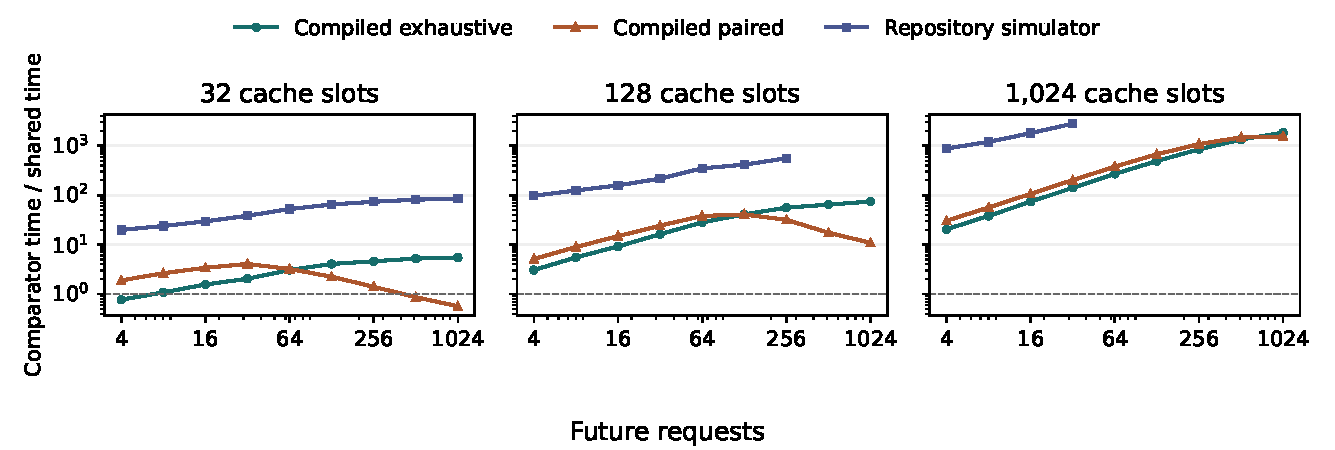
\includegraphics[width=0.92\linewidth]{labeler-benchmarks.pdf}
\caption{Recorded Phase 2B steady-state time ratios at capacities 32, 128 and 1,024. Values above one favor the shared labeler. Compilation and preparation are excluded. Some large configurations omit the reference Python comparator.}
\label{fig:benchmark}
\end{figure}

Median comparator/shared timing ratios were 19.7 for compiled exhaustive, 24.4 for compiled Phase 2A paired replay and 205.7 for the Python repository simulator. At \(C=32,H=4\) the shared and compiled exhaustive times were 6.92 and 5.31 microseconds per decision. The paired implementation allocates an \((H+1)\times C\) reference matrix. Python allocation tracing misses some native memory; process RSS includes runtime state. Figure~\ref{fig:benchmark} uses existing measurements.

\section{Phase 2A experiments}
The terminal core recorded 210 units. A reshape failure in exact byte grouping was repaired and resumed with 189 units preserved. The subsequent public-data census completed separately. The paired LRU study used 1,176 primary time-stratified and 504 separate learner-disagreement groups. In the primary sample, 99.76\% of 86,632 alternatives reached exact ordered coalescence, with the remainder reaching trace end. The mean consumed rollout was 79 requests and the maximum 1,163. Only 3.05\% of tested alternatives were profitable, touching 64 of the 1,176 states. The enriched sample's 37,128 alternatives had 1.55\% positives under a different sampling design. No cap-truncated branch was treated as fully resolved.

The forced-MIN census found 19.05\% all-tie groups and 84.39\% zero-regret candidate actions on average. Strict farthest-next labels excluded another optimal action in 884 of 1,176 states. A shortlist with LRU and seven alternatives can cover a common optimal action yet miss almost all positive advantage. K=8 LRU-tail covered 8 of 64 profitable states. Low frequency, ghost-informed, SIEVE-derived~\cite{sieve}, and a uniform sample covered 33, 34, 35 and 53. The K=4/8 oldest-candidate hindsight policies took 551,423 and 543,193 misses. The unrestricted hindsight reference recorded 507,593 versus 565,126 for LRU.

A bounded compression trial reduced 14,700 groups to 12,049 distinct input-target groups. Payload decreased by 16.69\%. Loss differences were zero and the maximum full-batch gradient discrepancy was \(4.89\times10^{-15}\). Weighting by multiplicity retains the full-batch objective. It permits different minibatch schedules and does not preserve recurrent histories if applied to a sequence.

\section{Phase 2B matched student experiments}
Phase 2B matched fitted Ridge and histogram gradient boosting on H8 and fully resolved advantage. The primary sample contained 1,176 states; low-frequency K=8 included LRU, with the same 26 causal legacy features and gate grids across arms. It was \code{DATA_LIMITED}: training folds held 10--31 resolved-positive shortlist states and validation folds 0--14. The feature ablation was gated off. Diagnostics at 1,176, 5,000 and 20,000 states found 33, 125 and 440 positive K=8 states. Supplemental labels were counted in memory. The primary stored archive retained 1,176 groups.

At H8, 591 states were all tied. Of those, 138 split under resolution. Resolved labels left 453 ties and exposed 64 profitable states, versus four at H8. H512 recovered the 64 with five remaining action-value disagreements. Low-frequency K=8 captured 37 of 74 achievable one-action miss savings and covered 33 of the 64 profitable states. Uniform seeds covered 54--60.

\begin{table}[ht]
\centering
\begin{tabular}{@{}lrr@{}}
\toprule
Matched Phase 2B policy & Misses & Relative reduction \\ \midrule
LRU & 565,126 & 0.000\% \\
Ridge H8 / resolved & 563,596 / 566,306 & +0.271\% / $-0.209$\% \\
Boosting H8 / resolved & 562,563 / 562,138 & +0.454\% / +0.529\% \\
Rate-matched random (resolved Ridge) & 563,876 & +0.221\% \\
DeepSets H8 calibrated approximate tie (seed 7) & 564,072 & +0.187\% \\
DeepSets H8 calibrated strict gate (seed 7) & 564,060 & +0.189\% \\
DeepSets H8 calibrated approximate tie (seed 19) & 564,161 & +0.171\% \\
\bottomrule
\end{tabular}
\caption{Phase 2B complete-grid totals. The calibrated checkpoint replays reuse November fits. The matched random policy uses a common intervention-rate target.}
\label{tab:phase2b}
\end{table}

The exact argmin and fixed 0.05 near-tie replays regressed for the two DeepSets seeds; validation-calibrated approximate ties, rounding and strict gates saved small numbers of misses. Calibrated replays required about 121--134 times LRU CPU in that harness. Resolved boosting's miss reduction came with 101.89 times LRU CPU. No resolved student passed the screen.

\section{Phase 2C-A supervision generation}
The seven producer tasks and reducer verified 420 partitions across 42 family-capacity cells. The design included 100,000 primary decision groups with exact 20,000 and 50,000 subsets, plus 2,688 diagnostics at capacities 256, 512 and 1,024. Compressed partitions occupied 0.252 GiB. Whole-group sampling and recorded inclusion probabilities support inverse-probability estimates. There were 557--1,968 positive shortlist groups in training folds at the largest budget and 0--945 in validation folds. MetaKV had two and Wiki2018 zero in their validation roles.

\begin{center}
\begin{tabularx}{\linewidth}{@{}Yrr@{}}
\toprule
Observed horizon & All-tie rate & Disagreement with resolved \\ \midrule
8 requests & 61.93\% & --- \\
32 requests & 53.01\% & --- \\
\(C\) requests & 50.27\% & --- \\
\(4C\) requests & --- & 0.012\% \\
\(C\) distinct objects (or observed end) & 49.90\% & 0.000\% \\
Resolved & 49.90\% & reference \\
\bottomrule
\end{tabularx}
\end{center}

On primary capacities, low-frequency K=8 covered 40.28\% of profitable states and captured 39.98\% of attainable gain. LRU-tail, SIEVE-derived and ghost-informed covered 15.46\%, 53.54\% and 40.78\%. Ten uniform seeds covered 86.53--87.97\%. Median effective rank increased from 2.85 (legacy) to 4.11 (compact history), 4.56 (decay) and 7.77 (expanded temporal). Median exact repeat input fractions were 96.63\% and 56.78\% in the legacy and expanded views. Finite-sample plug-in information can be inflated by unique signatures. Exact benefit-minus-risk reconstruction had zero discrepancies. This phase generated supervision and diagnostics.

\section{Phase 2C-B controlled learning experiments}
The reducer verified 231 fit components, 3,234 validation/outer replays, 14 chronological parity checks and 224 unique checkpoint files. Two-part targets add an estimator component in each fold. Every stage has seven successful task receipts and the aggregation job succeeded. The earlier Phase 2B records remain marked by origin in the combined table.

Stage A crossed four budgets with Ridge versus histogram boosting and H8 versus resolved targets. The 1,176-state historical set has different coverage. The 20k/50k/100k sets are nested. For matched larger-budget Ridge H8, 562,577, 565,138 and 562,330 misses show nonmonotonic scaling. Boosting H8 beat resolved at 100k (564,423 versus 565,993), while boosting resolved beat H8 at 1,176 (562,138 versus 562,584). Match architecture and sample before attributing a target effect.

Stage B selected the architecture per fold using validation, then compared horizons and feature groups. The matched selected-architecture F0 resolved portfolio gave 563,465 misses. Compact F2 history gave 562,064 (0.542\% below LRU). F3 decay, F4 ghost and F5 workload context gave 565,585, 575,307 and 587,719. F6 expanded history gave 563,436 at 139.90 times LRU CPU. Cleaned legacy and compact historical features therefore support different conclusions from expanding the feature count.

Stage C's benefit/risk portfolio gave 562,134 misses, 1,331 fewer than matched direct F0 resolved and 2,992 fewer than LRU. This comparison holds architecture selection, budget, representation and shortlist fixed. Uniform K=8 seeds gave 564,059, 564,654 and 564,396. Full-candidate scoring reused the shortlist-trained scorer and gate, recording 572,399, 1.287\% worse than LRU. The fixed-state uniform shortlist coverage was much stronger than these closed-loop gains.

\begin{figure}[ht]
\centering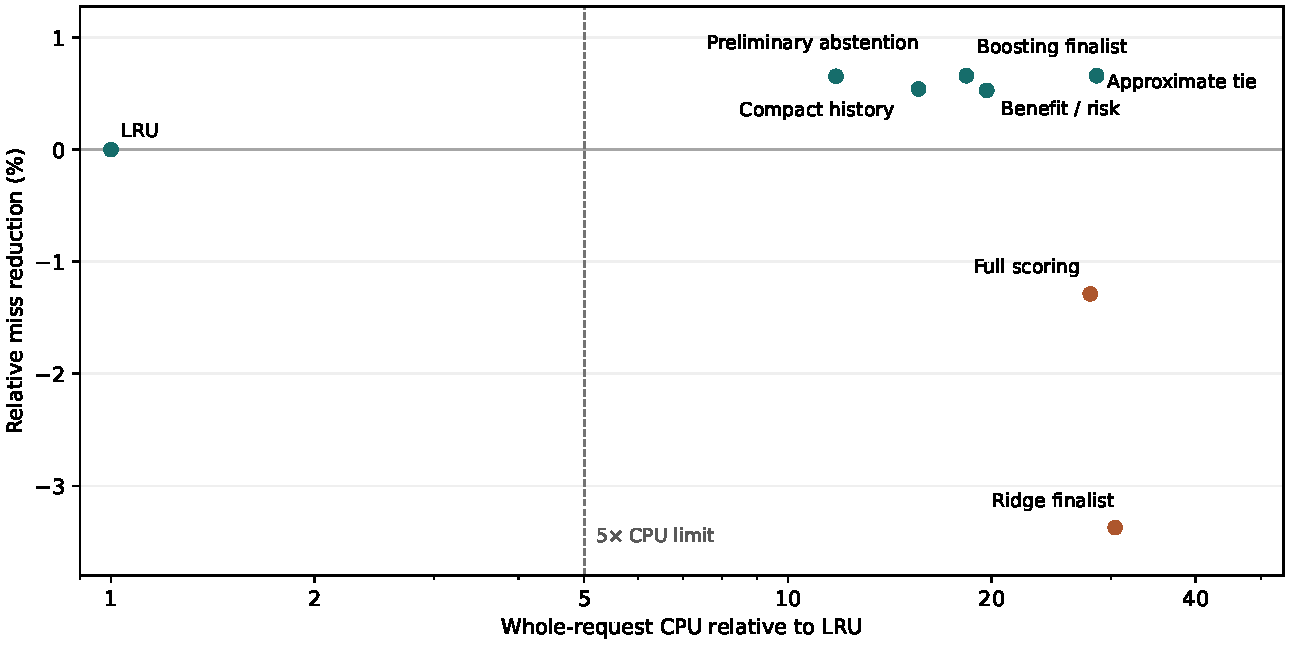
\includegraphics[width=0.93\linewidth]{finalist-tradeoffs.pdf}
\caption{Miss reductions and whole-request CPU overhead for selected complete-grid Phase 2C-B configurations. Each point uses the same LRU denominator for misses and the Phase 2C-B harness for CPU. The dashed line marks the provisional 5\(\times\) limit.}
\label{fig:tradeoff}
\end{figure}

\section{Conservative eviction and matched controls}
Stage D compared raw scoring, oldest exact tie, validation-calibrated approximate tie, and abstention. The strongest optimized boosting finalist gave 561,396 misses, a 0.660\% relative reduction (3,730 fewer misses) and a 0.444 percentage-point absolute reduction in miss ratio. Macro-family reduction was 0.560\%. The worst family, Citi Bike, regressed by 0.064\%, an increase of 30 misses. Excluding Alibaba Block leaves a reduction of 703 misses. All three primary capacities improved. The preliminary abstention version gave 561,424 misses at 11.78 times LRU CPU. The same-count approximate-tie configuration in the reducer took 28.57 times LRU, and the optimized finalist 18.35 times. Configuration identities and timings are kept separate in Figure~\ref{fig:tradeoff}.

Full-cache random, shortlist random, and gate-conditioned random controls each used five seeds. Validation-family intervention rates were set by capacity. Gate-conditioned random operates on its own trajectory and realized rates can differ. All 15 boosting controls lost to the boosting finalist, from 1,067 to 8,131 more misses. All 15 Ridge controls beat the Ridge finalist, by 5,698 to 14,742 misses. Deterministic budget-matched low frequency took 575,626 in the boosting comparison and 590,999 in the Ridge comparison. The Ridge finalist took 584,186. These controls distinguish selection of a victim from frequency of intervention while allowing state feedback.

The preregistered screen required at least 0.5\% relative reduction, positive macro and leave-one-family-out gains, at most 2\% regression in any family, an exact matched H8 comparison where applicable, advantage over matched controls, decision parity and CPU within 5 times LRU. The best boosting finalist passed the listed miss, family, controls and parity checks. Its reducer row has no exact matched H8 result, and its CPU exceeded the budget. Zero finalists passed all requirements.

\section{Computational efficiency and implementation costs}
Feature updates, shortlist formation, scoring, gating and cache transition were profiled in a common harness. Incremental request windows and preallocated feature buffers reduce materialization overhead. Ridge uses fused normalization and a direct dot product. Histogram boosting uses packed tree traversal with node-wise normalization. Reference versus optimized replays agreed on chronological decisions in all 14 recorded fold-finalist checks at capacity 64. Checks address parity for the tested policies, traces and capacity only. Aggregate optimized boosting CPU was 31.50 microseconds/request versus about 1.72 for profiled LRU. This corresponds to about 25 aggregate extra CPU seconds for 3,730 avoided misses, or 6.71 milliseconds of added CPU per avoided miss in these replays. That arithmetic uses process CPU and does not value actual cache misses or establish end-to-end benefit. Component clocks nest and should not be summed across levels. Memory observations combine resident metadata, bounded ghosts, and runtime allocations with differing scopes.

\section{Consolidated scientific findings}
The shared-stack derivation and comparator agreement establish a computational result for exact deterministic LRU supervision. Model fitting and policy replay remain separate bottlenecks. Compact history and separate benefit/risk estimation supported specific matched improvements. Approximate ties and selective intervention elicited a modest but measurable boosting advantage on the historical workloads.

Calibrated selective boosting outperformed its matched random controls on the retrospective grid, with heterogeneous gains and CPU cost beyond the provisional deployment limit. Ridge's ranking under random controls rules out the same interpretation for that finalist. Prior work establishes stack algorithms, optimal replacement and permutation-invariant modeling~\cite{mattson,belady,deepsets}. The shared evaluation derivation is documented with its assumptions and verification. Publication priority has not been established.

\section{Negative results and unsuccessful hypotheses}
Extra label discrimination and much larger samples did not yield uniform closed-loop gains. Richer features reduced observed aliasing but the corresponding lookup and temporal learners failed to improve policy outcomes consistently. Recurrent variants increased cost and miss counts. Full scoring and several deterministic and feature arms regressed. The final advancement screen remained unmet.

\section{Threats to validity}
\textbf{External validity.} The seven development lineages are retrospective, even under family-disjoint training. Capacity cells share requests. LAFC's reused lineages do not give independent replication. No independent confirmation or production deployment measurements exist for these candidates.

\textbf{Target validity.} Finite traces, fixed versus resolved observation windows, causal input limits and heavy ties affect what the targets measure. Repeated signatures are representation-specific. Sampling decisions by blocks and changing horizons or shortlists changes both measured rates and what gain means. Common-state counterfactuals and endogenous replays have different state distributions.

\textbf{Selection and measurement.} Validation can be sparse and favors abstention in some folds. Outer results are descriptive after the historical program explored many arms. Mean CPU includes harness-specific costs and depends on implementation, hardware, compilation and feature metadata coverage. Peaks and allocation tracing cover different memory surfaces. The single-action LRU guarantee has no extension here to arbitrary learned state or repeated overrides.

\section{Reproducibility and availability}
The companion repository package includes exact source snapshots, a per-file provenance ledger, curated aggregate CSVs, commands and data restrictions. The Phase 2C-B production SHA is recorded in the source ledger.\footnote{\code{59af9788394c25d026676302f133b2718459afa9}.} The source ledger records two portability edits to local paths and keeps the original Git blob identities. The approved aggregate archive is privately preserved with byte-level verification. Decision-level material, raw traces, checkpoints and restricted acquisition paths are held at their source. Independent confirmation remains sealed. Public reproduction of the tables and figures uses existing aggregates; exact numerical replay requires separately authorized source traces and pinned historical artifacts. The package's SHA-256 manifest covers the public deliverables.

\section{Final conclusions}
For deterministic LRU following a single forced victim choice, exact shared labels are computable in expected linear time in cache capacity plus suffix length. Their improved resolution is measurable and useful for auditing the learning task. The measured policy benefit is modest and workload-dependent. The finalist retained high CPU cost and failed the full advancement screen. The retained artifacts close the completed research record. The independent confirmation question remains open, and the scientific phase is closed.

\clearpage
\phantomsection
\addcontentsline{toc}{section}{References}
\bibliographystyle{plain}
\bibliography{references}

\appendix
\section{Reducer detail and final configurations}
\begin{table}[ht]
\centering
\begin{tabular}{@{}lrrrr@{}}
\toprule
Capacity & Requests & LRU misses & Boosting finalist & Saved \\ \midrule
32 & 280,000 & 194,269 & 193,498 & 771 \\
64 & 280,000 & 188,602 & 187,236 & 1,366 \\
128 & 280,000 & 182,255 & 180,662 & 1,593 \\
\midrule
All & 840,000 & 565,126 & 561,396 & 3,730 \\
\bottomrule
\end{tabular}
\caption{Phase 2C-B optimized boosting by capacity.}
\end{table}
\begin{table}[ht]
\centering
\begin{tabular}{@{}lrrr@{}}
\toprule
Family & LRU misses & Boosting finalist & Saved \\ \midrule
BrightKite & 40,048 & 39,746 & 302 \\
Citi Bike & 46,529 & 46,559 & $-30$ \\
Alibaba Block & 116,559 & 113,532 & 3,027 \\
MetaCDN & 67,745 & 67,314 & 431 \\
MetaKV & 91,660 & 91,660 & 0 \\
Twemcache & 82,585 & 82,585 & 0 \\
Wiki2018 & 120,000 & 120,000 & 0 \\
\bottomrule
\end{tabular}
\caption{Family-level aggregate counts, 120,000 scored requests per family.}
\end{table}

\begin{table}[ht]
\centering
\begin{tabular}{@{}lrrrr@{}}
\toprule
Stage & Configs/fold & Fits/fold & Replays/fold & Extra parity/fold \\ \midrule
A: Scaling & 16 & 16 & 96 & 0 \\
B: Horizons/features & 8 & 8 & 48 & 0 \\
C: Components/shortlists & 9 & 9 & 54 & 0 \\
D: Gates, controls and CPU & 44 & 0 & 264 & 2 \\
\bottomrule
\end{tabular}
\caption{Phase 2C-B reducer accounting, seven folds per stage. Parity is an implementation check on retrospective data. The 33 fit components per fold use 32 files.}
\end{table}

\section{Implementation settings}
\begin{tabularx}{\linewidth}{@{}p{0.22\linewidth}X@{}}
\toprule
Item & Configuration \\ \midrule
Runtime & Python 3.11.16, NumPy 2.3.5, Numba 0.65.0, scikit-learn 1.8.0, joblib 1.5.3. Single CPU per task. \\
Estimators & Ridge alpha 10, histogram boosting 30 iterations and depth at most 3. The exact model arguments and feature column lists are in the companion source and configuration. \\
Features & F0 legacy, F1 cleaned legacy, F2 compact history, F3 decay, F4 ghost, F5 selected workload context, F6 expanded temporal. Standardization is fitted inside the training role. \\
Gate grid & Strict improvement 0, .005, .01, .025, .05, .10, .20, .40 and always LRU. Approximate tie grid 0, .01, .025, .05, .10. Risk caps .25, .50, .75 and 1. \\
Controls & Random seeds 7, 19, 42, 101, 211. Uniform shortlist seeds 7, 19, 42. All shortlists retain the baseline victim. Fixed no-future candidate selection; hindsight controls reported separately. \\
Weighting & Equal training group weight with candidate weights scaled by \(8/K\). Wide-sample calibration uses inverse inclusion probability. The 1,176-group arm uses equal weighting. \\
\bottomrule
\end{tabularx}

\section{Evidence index}
\begin{itemize}
\item November terminal \code{replay_summary.csv} and Phase 1 terminal \code{RESULTS.md} supply neural and recurrent aggregate replays.
\item Phase 2A positive-horizon paired audits and forensic tables supply the tie, shortlist, census, censoring and compression diagnostics.
\item The Phase 2B aggregate manifest covers the labeler benchmark, correctness case counts and archived join checks.
\item Phase 2C-A reducer summaries supply design-weighted horizons, feature information, shortlist coverage and resource results. Phase 2C-B reducer \code{FINAL_POLICY_COMPARISON.csv}, family and capacity rows, criterion results and parity records supply the controlled comparison.
\item The repository evidence inventory records source revisions, dates, historical controls and access restrictions. Supplementary aggregate CSVs carry more configurations than appear in this report.
\end{itemize}
\end{document}
